\Titular*%
{De onde xorde a ecuación de Schrödinger?}%
{Mauro Garrido Rodríguez}%
{divulgacion}%
{Unha bela relación entre a mecánica clásica, a óptica e a cuántica.}%

\begin{refsection}
\begin{multicols}{2}


Na maioría de libros de texto de mecánica cuántica a ecuación de Schrödinger
introdúcese axiomaticamente; como é posible non dar unha xustificación da pedra
angular da cuántica? Como chegou Schrödinger á súa ecuación? Neste artigo imos
explorar o xeito, elegante e profundo, co que Schrödinger chega a unha das máis
importantes ecuacións da física no seu artigo de 1926, adaptándoo ao lector
para unha exposición máis didáctica.

\subsection*{A analoxía opto-mecánica}

Schrödinger lémbranos como, antes de ser coñecido o fenómeno da difracción da
luz, esta era considerada como transportada por <<raios>>: a luz propagábase en
liña recta nun mesmo medio, e cambiaba a súa pendente ao pasar a outros, mais
mantendo sempre unha propagación rectilínea. Se un físico que só coñecese a
óptica xeométrica (O.X.) quixese explicar a difracción, dinos Schrödinger,
atoparíase con que os raios \textit{xa non serían rectilíneos e influiríanse
uns aos outros dun xeito do máis curioso, en total contradición coas máis
fundamentais leis da óptica xeométrica}. Na macroescala a O.X. pode funcionar,
mais cando os obxectos cos que tratamos vólvense comparables coa lonxitude de
onda da luz (un parámetro que por suposto na O.X. carece de sentido) esta falla
estrepitosamente e temos fenómenos como os de difracción. A raíz disto, e
inspirado no traballo de De Broglie, dinos: \textit{acaso non está un tentado a
investigar se a non-aplicabilidade da mecánica ordinaria a problemas
micromecánicos é quizais do mesmo tipo que a non-aplicabilidade da óptica
xeométrica no fenómeno de difracción ou interferencia?}. Hai acaso unha
formulación da mecánica clásica que teña que ver cun comportamento ondulatorio?
\textbf{Si}, e era coñecida por \textbf{sir William Rowan Hamilton} en 1833.
Este fixouse no parecido do principio de mínima acción mecánico co principio de
Fermat óptico. Lembremos que di cada un:

\begin{itemize}

    \item \textbf{Principio de mínima acción}. Resumidamente, consiste nunha
reformulación da mecánica clásica (a chamada mecánica analítica), onde, de
tódalas traxectorias posibles que pode tomar un partícula, esta só escolle
aquela que fai estacionaria unha determinada cantidade denominada
\textbf{acción} (isto é, que non cambia a primeira orde baixo variacións
pequenas da traxectoria), de xeito que

    \begin{equation}
        \delta S = 0 \rightarrow \frac{d}{dt}\frac{\partial
        \mathcal{L}}{\partial \Dot{q}} - \frac{\partial\mathcal{L}}{\partial q} = 0
    \end{equation}

    onde $\mathcal{L} = T-V$ é o lagranxiano,
$S=\int_{t_0,q_0}^{t,q}\mathcal{L}(q,\Dot{q},t)dt$, e a ecuación que se deriva
do principio de mínima acción é a ecuación de Euler-Lagrange, que é a que rexe
o movemento da partícula, o equivalente a $F=ma$ na mecánica estándar ou
clásica.

    \begin{figure}[H]
       \centering
       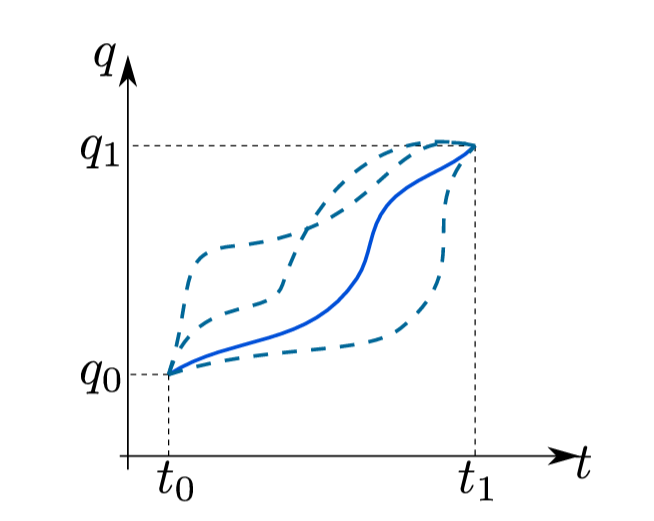
\includegraphics[width=0.7\linewidth]{revistas/002/imaxes/hj2.png}
       \caption{Traxectorias posibles para unha partícula (Fonte: \cite{bahramhouchmandzadeh_2020})}
    \end{figure}

    \item \textbf{Principio de Fermat}. Postula que os raios de luz seguen as
traxectorias de mínimo tempo. Lagrange xeneralizaríao matizando que realmente
as traxectorias que son escollidas son as estacionarias. Ao igual que no caso
mecánico, non sempre se escollen as traxectorias de mínima acción, senón as que
a fan estacionaria. Este principio, de feito, pode facerse equivalente ao
anterior tendo en conta un lagranxiano óptico $\mathcal{L_{op}} = n(s)$ ($n(s)$
é o índice de refracción en cada punto), sendo a nosa condición de <<acción
óptica>> ou <<camiño óptico>> estacionario a seguinte
    \begin{equation}
        \delta S_{op} = \int_A^B\mathcal{L_{op}}ds = 0
    \end{equation}

    Este camiño óptico ten unha interpretación clara: é a distancia que
recorrería a luz no baleiro no tempo que tarda esta en facelo nun medio con
$n(s)$, posto que o índice é unha medida da relación entre as distancias
percorridas nun medio e no baleiro, $n=\frac{c}{v} = \frac{dx_c/dt}{dx_v/dt} =
\frac{dx_c}{dx_v}$. Se resolvemos esta ecuación, atoparemos a \textbf{ecuación
dos raios da óptica xeométrica}.
    \begin{equation}
        \frac{d}{ds}(n\frac{d\vec{r}}{ds})=\nabla n
    \end{equation}

    Así, esta analoxía levou a Hamilton á idea de que o movemento dunha
partícula podería describirse como o análogo a un raio de luz propagándose nun
medio inhomoxéneo ($n(s)$).

    Así, \textbf{de igual xeito que os raios ópticos seguen liñas ortogonais ás
superficies de fase constante} (as frontes de onda da luz), \textbf{as
traxectorias das partículas seguirían liñas ortogonais ás superficies de acción
constante}. A partir desta profunda idea, Hamilton propón que
    \begin{equation}
        p=\frac{\partial S}{\partial q}
    \end{equation}

\end{itemize}

É dicir, que a variación da acción coa posición (xeneralizada) dá lugar ao
momento (xeneralizado) das partículas, que polo tanto se moven ortogonalmente
ás superficies de acción constante.

\begin{figure}[H]
   \centering
   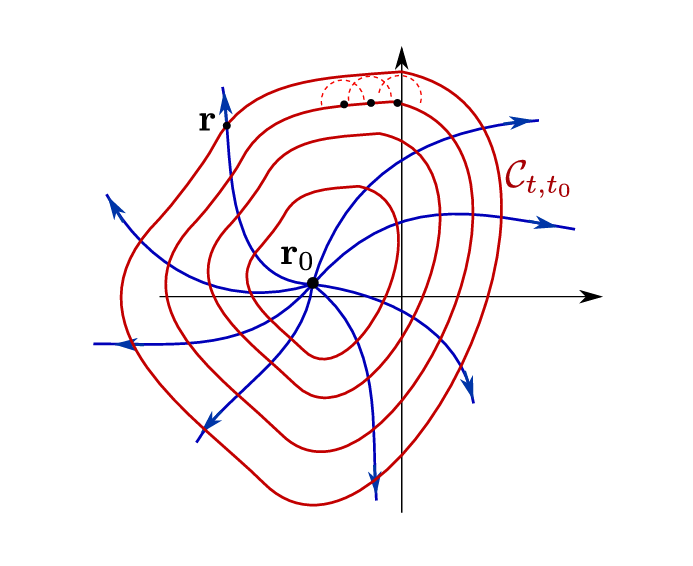
\includegraphics[width=0.6\linewidth]{revistas/002/imaxes/hj1.png}
   \caption{Relación entre as superficies de fase constante e os raios (Fonte: \cite{bahramhouchmandzadeh_2020})}
\end{figure}

Se combinamos este feito co principio de mínima acción, pasando primeiro polas
\textbf{ecuacións canónicas} (reformulación da de Euler-Lagrange facendo o
cambio de dependencia $\Dot{q}\rightarrow p$, onde agora o papel de
$\mathcal{L}$ faino $\mathcal{H}$, o Hamiltoniano), atopamos a ecuación de
\textbf{Hamilton-Jacobi}.

\begin{equation}
    \frac{\partial S}{\partial t} + \mathcal{H}(q,\frac{\partial S}{\partial q},t) = 0
\end{equation}

Esta ecuación, aínda que non o pareza, é clave para entender a ecuación de
Schrödinger. Imos reescribila e ver o caso máis simple para entendela mellor, o
dunha partícula de masa $m$ movéndose nun potencial $V(x,y,z)$, de xeito que
$\mathcal{H}=E=T+V=\frac{1}{2m}(p_x^2+p_y^2+p_z^2) + V(x,y,z)$. Se incluímos
este hamiltoniano na ecuación de Hamilton-Jacobi, e tendo en conta a suposición
de Hamilton $p=\frac{\partial S}{\partial q}$ atopamos que

\begin{equation}
    \frac{\partial S}{\partial t} + \frac{|\nabla S|^2}{2m} + V(x,y,z)=0
\end{equation}

Para simplificar aínda máis esta expresión consideremos un hamiltoniano
independente do tempo, de xeito que obteñamos unha ecuación para partículas con
enerxía constante. Isto determinará a dependencia temporal da acción

\begin{equation}
    \frac{\partial S}{\partial t} = -\mathcal{H} \rightarrow
    \boxed{S=(E)t + f(x,y,z)}
\end{equation}

Deste xeito, executando a derivada temporal de $S$, a ecuación de
Hamilton-Jacobi queda reducida a

\begin{equation}
    |\nabla S| = \sqrt{2m(E-V)}
\end{equation}

Posto que a enerxía cinética é $T=E-V$, isto non é máis que

\begin{equation}
    |\nabla S| =  |\vec{p}| \rightarrow \boxed{\nabla S = \vec{p}}
\end{equation}

O gradiente da acción, perpendicular ás traxectorias, é o momento da partícula.
Esta é a ecuación dos raios-mecánicos, é dicir, das traxectorias, de enerxía
constante.

\subsection*{A analoxía opto-mecano-cuántica}

Schrödinger é consciente de que ata aquí non hai nada novo. O que el propón é
tomarse esta ecuación en serio. Se realmente esta é o equivalente á ecuación
dos raios da O.X., e a óptica é en realidade ondulatoria, emerxendo estes
delas, por que non facer o mesmo para as partículas, para as súas traxectorias?
Tomándonos en serio a analoxía, a ecuación de Hamilton-Jacobi asócialles ás
partículas unha fase, a acción, que debe de ser a fase dunha onda. \textbf{Se a
luz cumpría unha determinada ecuación de ondas, que ecuación de ondas cumprirá
unha partícula material?}

Antes de chegar a ela, temos que ter en claro que tipo de onda é a que ten a
fase da ecuación de Hamilton-Jacobi: posto que provén de esixir unha fase
estacionaria, pódese probar moi facilmente que é equivalente á \textbf{ecuación
da \textit{eikonal}} da óptica, que é válida para \textbf{ondas
localmente planas}, é dicir, ondas cunha variación de fase suave, con frontes
de onda localmente planas.

\begin{figure}[H]
   \centering
   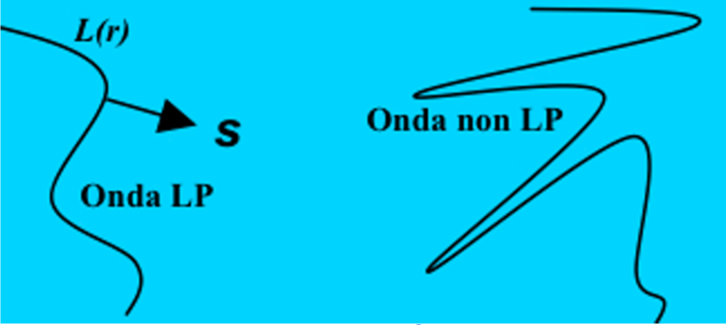
\includegraphics[width=0.7\linewidth]{revistas/002/imaxes/hj3.png}
   \captionof{figure}{Ondas localmente planas (Fonte: \cite{apuntes_optica_2})}
\end{figure}

Na mecánica clásica as únicas ondas consideradas serán localmente planas, que dan
solucións exactas para as traxectorias; pero, en mecánica cuántica, ao igual
que pasaba coa óptica ondulatoria e coa O.X., poderemos ter moitas máis
posibilidades de ondas, \textbf{que darán lugar a movementos inexplicables
mediante o concepto de raios, é dicir, de traxectorias}.

Así, antes de pasar á ecuación de Schrödinger, poremos a proba este concepto de
ondas asociándolle á función de ondas $\Psi$ (o que ondula, cuxo significado
descoñecemos, análogo ao campo electromagnético da luz) dunha \textbf{onda
localmente plana} (polo comentado de que a ecuación de Hamilton-Jacobi só
aplica a estas) a acción $S = Et + f(x,y,z)$ como fase (lembremos que isto
implica E=cte), recordando que debe cumprir $\nabla S=\vec{p}\rightarrow \nabla f(x,y,z) = \vec{p}$. Así,
\begin{equation}
    \Psi = A(x,y,z)e^{i(\frac{S}{B})} = A(x,y,z)e^{i(\frac{E}{B}t + f(x,y,z)/B)}
\end{equation}

onde $B$ é unha constante que permite que o que entra na exponencial sexa
adimensional. Esta é a clase de ondas que corresponden á ecuación de
Hamilton-Jacobi, ondas localmente planas de $E=cte$ cuxas frontes son moldeadas
por $f(x,y,z)$.

Schrödinger di: \textit{un non pode resistir a tentación de supor que $B$ sexa
unha constante universal, porque nese caso}, facendo $B=\hbar$, a frecuencia
desta onda é

\begin{equation}
    \omega=\frac{E}{\hbar} \rightarrow \boxed{E=\hbar \omega}
\end{equation}

A famosa relación de De Broglie enerxía-frecuencia!

\subsection*{A ecuación de Schrödinger}

Para o caso simple que estamos tratando da partícula unidimensional,
Schrödinger propón que $\Psi$ cumpre unha ecuación de ondas ordinaria

\begin{equation}
        \frac{\partial^2 \Psi}{\partial x^2} =
        \frac{1}{u^2}\frac{\partial^2 \Psi}{\partial t^2}
\end{equation}

Agora, asume que estas ondas se moven cunha velocidade de fase dada pola
ecuación de Hamilton-Jacobi ($p=\frac{\partial S}{\partial x} \rightarrow v=
\frac{1}{m} \frac{\partial S}{\partial x}$), asumindo tamén solucións de
enerxía constante (polo tanto, a parte temporal da acción será $S=Et$), o cal
converte a esta ecuación de ondas na \textbf{ecuación de Schrödinger
independente do tempo}. Así,

\begin{equation}
    \boxed{
        -\frac{\hbar}{2m}\frac{\partial^2\Psi}{\partial x^2} +
        V(x,y,z)\Psi = E\Psi
    }
\end{equation}

Que, polo dito anteriormente, é unha ecuación só válida para ondas asociadas a
partículas de enerxía constante. Fixémonos en que agora non se asume unha onda localmente
plana (a ecuación non foi obtida con esa premisa), co que esta ecuación é
valida para ondas arbitrarias que corresponderían ás <<traxectorias>>
cuánticas. Plasmar a importancia desta ecuación neste artigo é unha tarefa
colosal que non pode abarcarse aquí, mais o que fai Schrödinger inmediatamente
despois de conseguila é aplicala ao átomo de Hidróxeno, reproducindo así os
valores cuantificados dos niveis de enerxía, explicando o átomo de Bohr. É de
interese resaltar o feito de que se poidan obter tantos resultados sen darlle á
$\Psi$ unha interpretación aínda.


\nocite{schrodinger.e_1926}
\nocite{schrodinger.e_1926_2}
\nocite{hamilton_optico_mechanical}
\nocite{hamilton_jacobi_equation}

\printbibliography

\end{multicols}
\end{refsection}
